\begin{figure}[H]
  \centering
  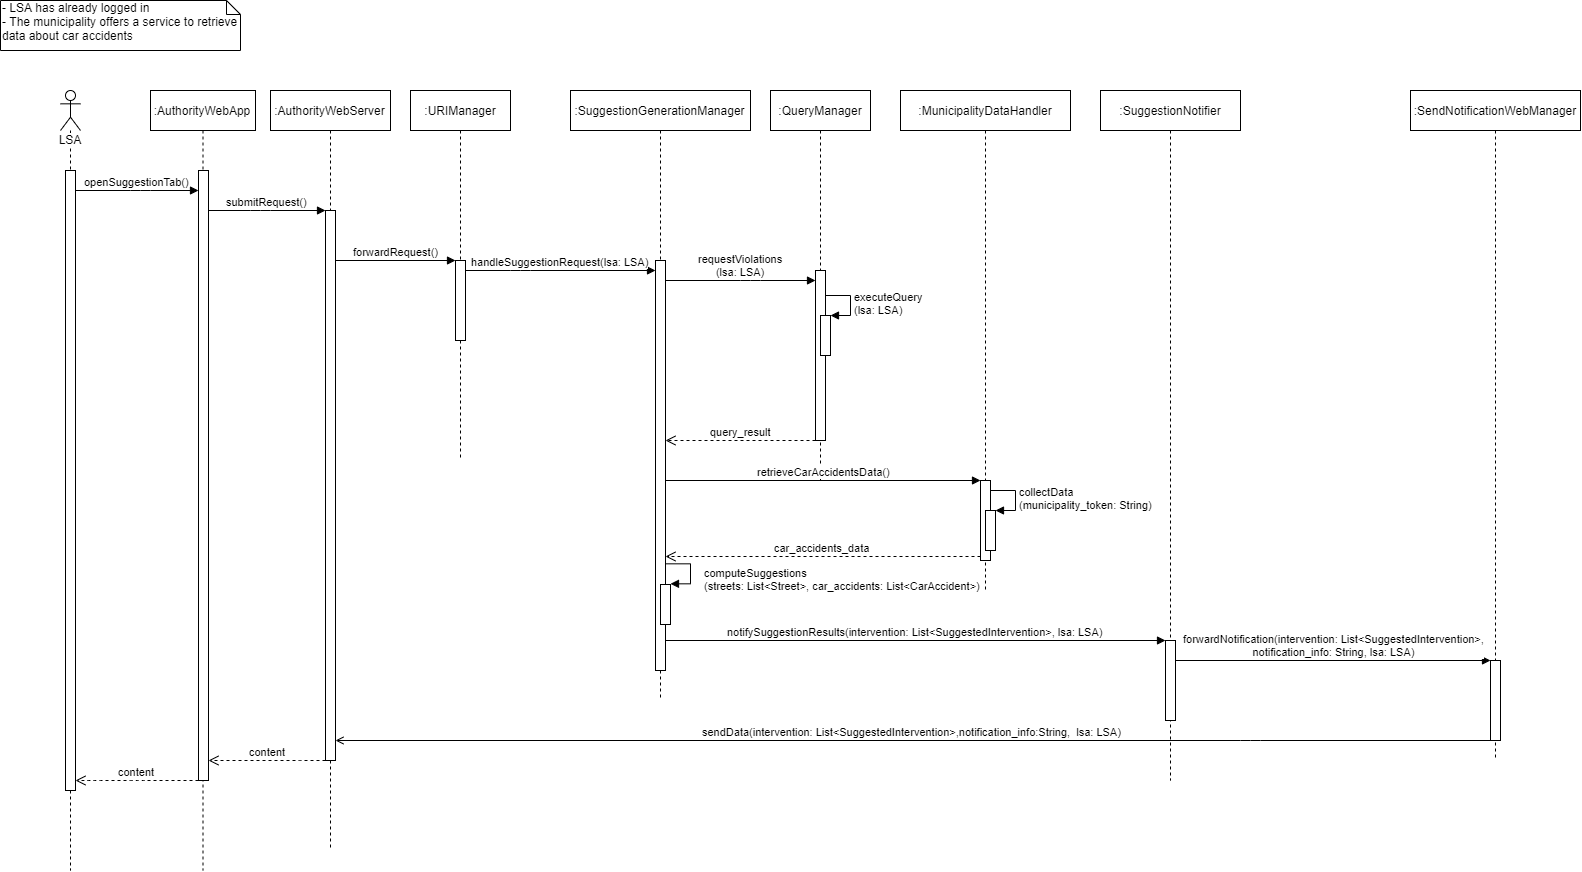
\includegraphics[width=1\textwidth]{Images/UML_diagrams/Sequence_Diagrams/Ask_for_suggestions_sd.png}
  \caption{Ask for suggestions sequence diagram}
  \label{fig:ask_suggestions_sd}
\end{figure}
This last sequence diagram describes the advanced functionality of creating suggestions by crossing violation reports with the car accidents data provided by the municipality. The LSA that wants to retrieve suggestion that can possibly be made in his competence area, submits a request via the web app. As always the request arrives to the URIManager via the AuthorityWebServer and then it is routed to the SuggestionGenerationManager that will have to perform this three actions in order:
\begin{enumerate}
  \item Send a request to the QueryManager to perform a query that provides with the most frequent categories of violations, and the related streets in the LSA competence area;
  \item Once query result is provided, forward a request to the MunicipalityDataHandler that will automatically collect the car accidents data by retrieving it from the MunicipalityDataSharing component;
  \item Once all the necessary data are provided, cross the information and generate a list of suggested intervention. 
\end{enumerate}

If some suggestions have been found, they are sent over to the SuggestionNotifier that will forward them to the SendNotificationWebManager, that in its turn will send them back to the LSA web application. As a side note about the MunicipalityDataSharing; here it is not represented the process of asking data to the external municipality system done by the MunicipalityDataHandler as it is, for the sake of simplicity, embedded into a function called by the MunicipalityDataHandler itself. 
% TODO: is last part good enough ?
